\chapter{采样作为数值求解：DDIM、DPM 与 EDM}
\label{th:solvers}

\section{要区分模型误差与积分误差}

概率流 ODE 为 $\dot x=u_\theta(x,t)$。
真实速度与 $u_\theta$ 的差是模型误差；
用有限步近似这个已学速度场的误差是数值误差。
高阶求解器可以减少后一项，不能自动修复错误条件、模型覆盖不足或 codec 丢失。

若速度足够光滑且 Lipschitz，Euler 的单步局部截断误差为 $O(h^2)$，
固定区间的全局误差通常为 $O(h)$。
Heun 用两次速度估计：
\begin{align}
k_1&=u_\theta(x_t,t),\qquad \tilde x=x_t+h k_1,\\
k_2&=u_\theta(\tilde x,t+h),\qquad
x_{t+h}=x_t+\tfrac h2(k_1+k_2).
\end{align}
它在对应光滑条件下全局二阶，通常每步2次网络求值。
生成使用 $h<0$，这不改变确定性积分阶数的基本分析。

\begin{figure}[htbp]
\centering
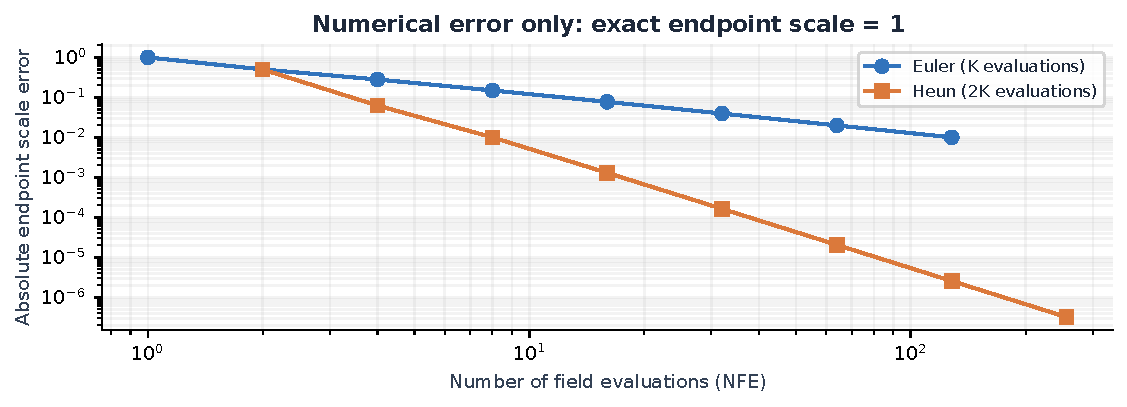
\includegraphics[width=0.84\linewidth]{assets/theory/solver-error.pdf}
\caption{在已知解析速度 $u_t(x)=(2t-1)x/((1-t)^2+t^2)$ 上，
从噪声1反向积分到数据0，比较端点缩放误差。横轴按网络求值次数计。
这仅隔离数值积分误差，没有神经网络误差，也不是性能基准。}
\end{figure}

\section{ODE 高阶与 SDE 高阶不能混为一谈}

反向 SDE 若用正向反时钟写为 $\mathrm dY=b\mathrm dr+g\mathrm dB$，
Euler--Maruyama 更新是
$Y_{n+1}=Y_n+b(Y_n,r_n)h+g(r_n)\sqrt h\,z_n$。
一般条件下常讨论强阶 $1/2$、弱阶1；
加性噪声等特殊结构可改善阶数，不能把它们当对所有 SDE 的统一结论。
给 Heun ODE 更新随意加噪，不会自动变成同阶的 SDE 求解器。

步数减少还会改变随机路径的近似与终端分布，
比较采样器时应固定输出参数化、时间表、guidance、起始噪声分布与解码器。

\section{DDIM 的确定与随机更新}

DDIM 允许保持同一 $q(x_t\mid x_0)$ 的同时采用不同联合路径。
记 $t>s$ 为两层离散噪声时刻，$a_t=\sqrt{\bar\alpha_t}$，
$b_t=\sqrt{1-\bar\alpha_t}$，先预测
$\hat x_0=(x_t-b_t\epsilon_\theta)/a_t$，再更新
\begin{equation}\label{th:ddim}
x_s=a_s\hat x_0+\sqrt{b_s^2-\xi_{t,s}^2}\,\epsilon_\theta(x_t,t)
 +\xi_{t,s}z.
\end{equation}
常取
\[
\xi_{t,s}=\eta\sqrt{\frac{1-\bar\alpha_s}{1-\bar\alpha_t}}
 \sqrt{1-\frac{\bar\alpha_t}{\bar\alpha_s}},\qquad0\leq\eta\leq1.
\]
$\eta=0$ 时为确定映射；相邻原时间步、相容方差设置下 $\eta=1$ 可联系 DDPM。
不能不加条件地把任意跳步 $\eta=1$ 宣称为原始训练链的逐步 DDPM。

确定 DDIM 不是“每步都直接输出干净预测”；它保留了到目标噪声级的残余噪声方向。
DDIM 反演与生成互逆只在精确连续动力学或特殊离散条件下成立，
有限步近似反演会有重建误差。

\section{积分因子揭示扩散专用求解器}

在 $a_t,b_t>0$ 的区间，用噪声预测重写概率流：
\[
\dot x_t=\frac{\dot a_t}{a_t}x_t+
 \left(\dot b_t-\frac{\dot a_t}{a_t}b_t\right)\epsilon_\theta(x_t,t).
\]
取 $\lambda=\log(a/b)$，对积分因子 $x/a$ 求导，得到
\begin{equation}\label{th:dpm-integral}
x_s=\frac{a_s}{a_t}x_t
 -a_s\int_{\lambda_t}^{\lambda_s}
 e^{-\lambda}\epsilon_\theta(x(\lambda),t(\lambda))\,\mathrm d\lambda.
\end{equation}
反向生成时 $\lambda_s>\lambda_t$。
冻结区间内噪声预测可精确积分指数权重，得到
\[
x_s=\frac{a_s}{a_t}x_t-
 a_s(e^{-\lambda_t}-e^{-\lambda_s})\epsilon_\theta(x_t,t),
\]
即 $a_s\hat x_0+b_s\epsilon_\theta$ 的确定 DDIM 形式。
所以 DDIM 可解释为特定积分变量下的一阶指数型求解，
不应笼统称为任意时间坐标上的普通 Euler。

DPM-Solver 对该积分中神经网络项作更高阶近似；
DEIS 也利用半线性结构与指数积分，但系数和插值构造需要各自定义。
线性部分精确处理不代表非线性项或网络误差也消失。

\section{DPM-Solver++ 与数据预测形式}

把 ODE 改写为 $\hat x_0$ 预测，并对 $x/b$ 使用积分因子：
\begin{equation}\label{th:dpmpp-integral}
x_s=\frac{b_s}{b_t}x_t+
 b_s\int_{\lambda_t}^{\lambda_s}e^\lambda\hat x_{0,\theta}(x(\lambda),t(\lambda))
 \,\mathrm d\lambda.
\end{equation}
一阶冻结预测给出 $(b_s/b_t)x_t+(a_s-a_tb_s/b_t)\hat x_0$，
同样与确定 DDIM 一致。高阶时，对噪声函数还是数据函数插值会产生不同数值性质。
DPM-Solver++ 强调有引导采样的稳定性，不能只把名字中的“++”当作所有设置必胜。

多步法复用过去预测，启动时需要低阶步骤；提示改变、时间表改变或强非光滑裁剪
都可能破坏其高阶近似假设。动态 threshold 对像素范围的意义，
也不能不作变换就应用于无界潜变量。

\section{EDM 的噪声尺度求解}

在 $y=x_0+\sigma\epsilon$ 的坐标中，
去噪器 $D_\theta(y,\sigma)$ 给出 ODE
\begin{equation}\label{th:edm-ode}
\frac{\mathrm dy}{\mathrm d\sigma}=\frac{y-D_\theta(y,\sigma)}{\sigma}.
\end{equation}
可用 Euler 预测与 Heun 校正。若下一步 $\sigma=0$，
通常直接用最终 Euler/去噪端点，避免计算除零的第二次斜率。
常见噪声网格为
\[
\sigma_i=\left[\sigma_{\max}^{1/\rho}
 +\frac i{K-1}(\sigma_{\min}^{1/\rho}-\sigma_{\max}^{1/\rho})\right]^\rho,
\quad i=0,\ldots,K-1,
\]
再另加终点0。$\rho$ 改变步长分配，是数值选择而非新概率模型。
EDM 的 churn 在指定噪声区间先增噪再去噪，有独立超参数与质量权衡。

\section{NFE、并行与自适应的真实口径}

两分支 CFG 的 $K$ 步 Euler 包含约 $2K$ 次样本级网络求值；
Heun 再按校正次数增加。合成一个 batch 改变吞吐，不消除算术量。
多步法可在启动后每步1次求值，高阶单步法可能每步需要多次。
自适应求解器还有被拒绝步骤；统计只接受的步骤会低估成本。

并行 Picard 一类方法通过预测整段轨迹并迭代校正减少串行深度，
不是把状态依赖的每一步直接独立并行。应计入迭代、冗余计算与停止误差。
端到端时间还含文本编码、codec 与后处理；NFE 是重要口径，不是完整运行时间。

\begin{theorytakeaway}
采样器必须匹配模型的概率路径、输出和端点。
改进求解器是更好地积分一个给定场，蒸馏则改变被训练的映射；二者不能互相冒充。
\end{theorytakeaway}
\threading{主参考第9章\cite{theorybook}，DDIM、DPM-Solver、DPM-Solver++ 与 EDM
分别参见\cite{ddim,dpm,dpmpp,edm}。本章保留关键积分式，并明确时间与 log-SNR 约定。}
